\chapter{Desarrollo}
Recordemos de la Figura \ref{fig:diagrama_bloques_objetivo} que nuestro sistema está compuesto por 5 bloques. En este capítulo vamos descomponer y analizar cada bloque para su posterior implementación en la simulación.

\section{Análisis}
\subsection*{Codificador y Modulador}
Estos bloques son en realidad bastante simples. Consta de la sumatoria de dos señales sinusoidales. Para la simulación serían dos generadores establecidos en la combinación de frecuencias que corresponden a un determinado digito. Para crear la codificación, basta con ingresar ambas señales a un sumador. Esto luego debe sumarse a una señal constante de 1, con el fin de poder hacer el producto de la señal resultante con la señal portadora. El resultado de esto es la señal ya modulada, como se muestra en la Figura \ref{fig:bloques_cod_mod}.

\begin{figure}[H]
  \centering
  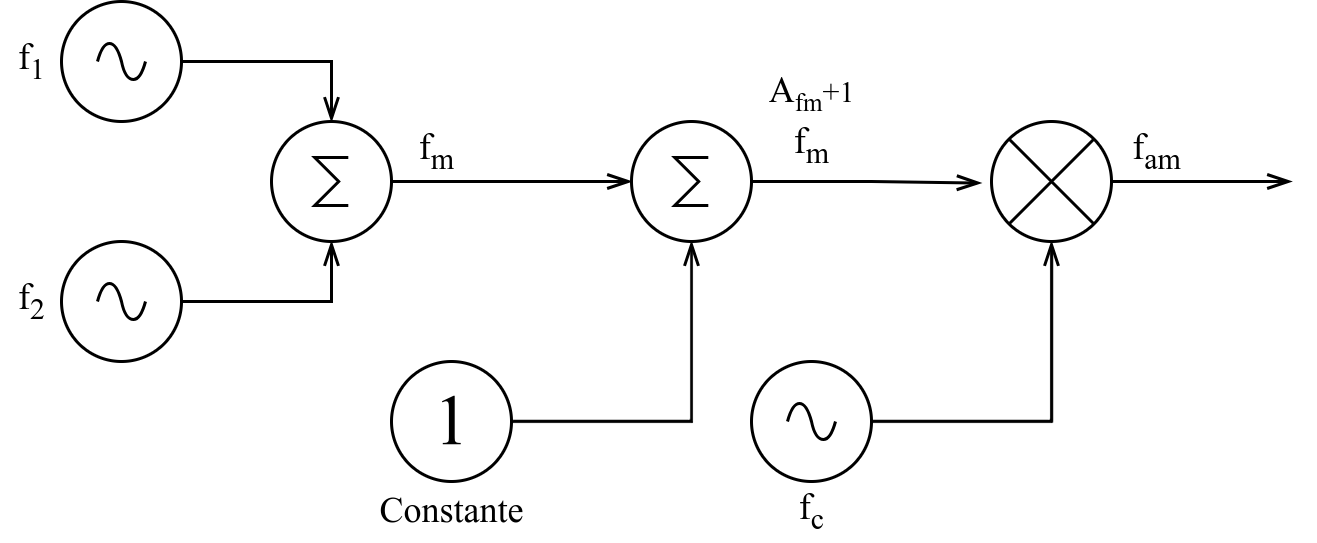
\includegraphics[width=400pt]{images/diagramas-codificador-modulador.png}
  \caption{Codificador y Modulador}
  \label{fig:bloques_cod_mod}
\end{figure}

\subsection*{Transmisión}
La transmisión será simulada a través de un filtro pasa-banda, estableciendo las frecuencias de corte de tal forma que el ancho de banda sea el espectro audible por el oído humano, como muestra la Figura \ref{fig:bloques_txs}.

\begin{figure}[H]
  \centering
  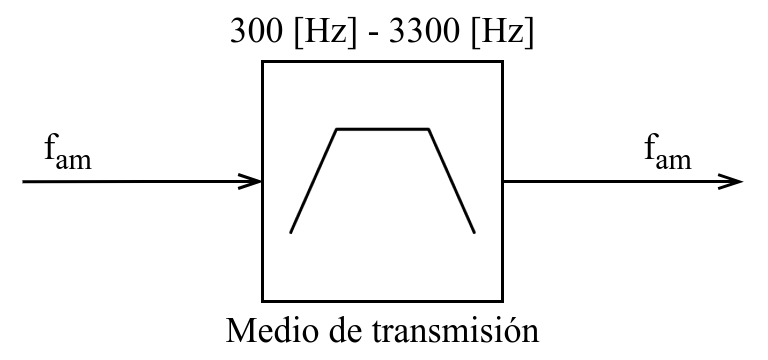
\includegraphics[width=300pt]{images/diagramas-transmision.png}
  \caption{Transmisión}
  \label{fig:bloques_txs}
\end{figure}

\subsection*{Demodulador}
Para demodular la señal, basta con realizar nuevamente el producto con la señal portadora. Como resultado obtenemos la frecuencia moduladora (que es la señal codificada, suma de las frecuencias que componen a un digito específico) como muestra la Figura \ref{fig:bloques_demod}. Luego debemos aplicar un filtro pasa bajos para limpiar la señal de ruidos que puedan haberse introducido, entre esos, algunos vestigios de la señal portadora.

\begin{figure}[H]
  \centering
  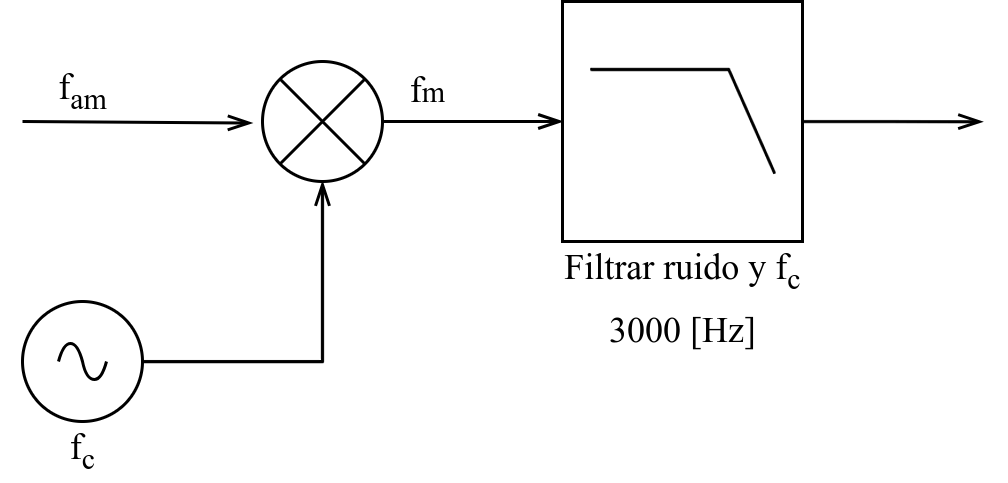
\includegraphics[width=350pt]{images/diagramas-demodulador.png}
  \caption{Transmisión}
  \label{fig:bloques_demod}
\end{figure}

\subsection*{Decodificador}
El bloque decodificador es el más complejo de todos, ya que este tiene la lógica para detectar las señales que componen la señal codificada. Como ya vimos en la Figura \ref{fig:diagrama_bloques_decod}, necesitamos 7 filtros pasa-banda para aislar cada una de las frecuencias de la matriz \gls{dtfm}, luego viene la matriz decodificadora. En la Figura \ref{fig:bloques_decod} vemos una simplificación de cómo estaría compuesta esta lógica de decodificación. Cada salida de control es una compuerta AND que se activara cuando sus dos entradas se encuentren activas (o en "1" lógico). Entonces cada compuerta representa la combinación de tonos para detectar cuál fué el digito enviado.

\begin{figure}[H]
  \centering
  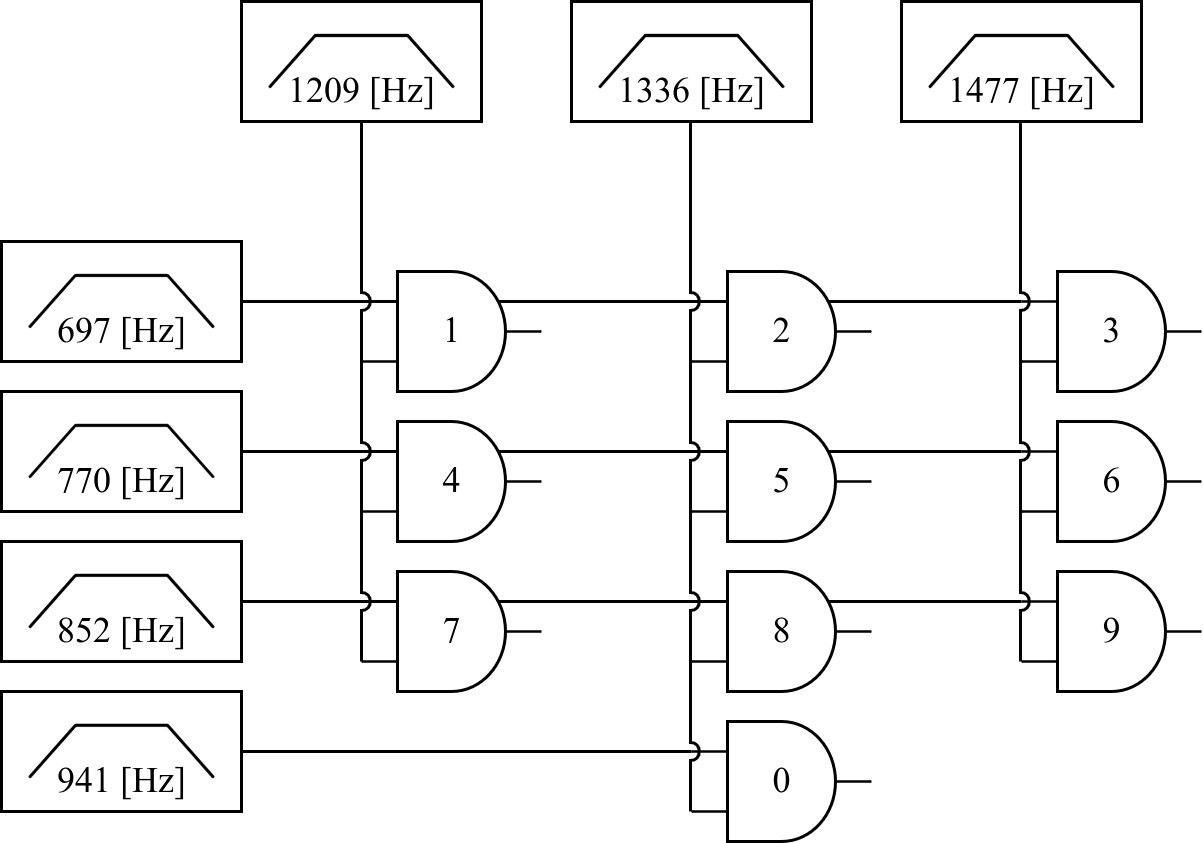
\includegraphics[width=350pt]{images/diagramas-decodificador-matriz.png}
  \caption{Decodificador}
  \label{fig:bloques_decod}
\end{figure}


\section{Diseño}
Como mencionamos en la sección anterior, para poder implementar los filtros digitales del banco de filtros del bloque decodificador, necesitamos emplear la herramienta fdatool del MATLAB, ya que estos filtros serán de muy alto orden lo que es engorroso para el cálculo analítico. En la interfaz de la herramienta

\section{Especificaciones}

\section{Prototipo}